\documentclass[conference,10pt]{IEEEtran}
\usepackage[T1]{fontenc}
\usepackage{amsmath,amssymb,booktabs,array,url,graphicx}
\usepackage{xurl}
\usepackage{hyphenat}
\usepackage[hidelinks]{hyperref}

\setlength{\emergencystretch}{1em}
\hypersetup{pdftitle={Healthy but Unsafe: How IT Agent Recoveries Undo Operator Work: Separating Configuration Safety, Reporting Evidence, and Live Service Recovery}}
\title{Healthy but Unsafe: How IT Agent Recoveries Undo Operator Work\\[0.3em]{\large Separating Configuration Safety, Reporting Evidence, and Live Service Recovery}}
\author{\IEEEauthorblockN{Santosh Sibyala}\IEEEauthorblockA{ORCID: 0009-0000-5970-4166\\santoshsibyala@gmail.com}}
\begin{document}
\maketitle


\begin{abstract}

When an IT agent recovers from a failed change, restoring the configuration value is only part of the job. The agent can overwrite work another operator did in the meantime, leave the service unhealthy, or report success without supporting evidence. We study these failures across controlled recovery tasks, running HTTP services, conventional compensation policies, and model\hyp{}driven execution. We distinguish four outcomes: whether existing work was preserved, how far recovery progressed, whether the final report was supported, and whether the service ended up healthy. In matched running\hyp{}service controls, full atomic checks, which combine ownership with cross\hyp{}resource predicates, produced no recovery\hyp{}history violations across 48 trajectories. Field\hyp{}level compensation and ownership\hyp{}only checks each produced 6 violations in 48, yet all three recovered the same number of configurations safely. In a preliminary Kubernetes validation, unsafe recoveries still passed health checks and produced completion reports that the evidence did not support, while ownership\hyp{}aware recovery kept operator work intact. In two 50-run cohorts, two tested LLM agents never re\hyp{}read the Deployment before writing; their unsafe recoveries passed health checks with unsupported reports. Two reviewers independently judged reporting support in 32 selected trajectories and agreed on 31 (Cohen's kappa = 0.95, or 0.88 when 14 error\hyp{}only records are excluded). The study uses small local applications, controlled interference, and a selected annotation sample, which limits generalization. These results show that restoring a value, preserving others' work, producing a supported report, and keeping a service running are separate outcomes, and each needs to be measured on its own.

\end{abstract}

\begin{IEEEkeywords}

IT operations, LLM agents, recovery, compensation, concurrency, evidence, evaluation.

\end{IEEEkeywords}

\section{Introduction}

By the time an IT agent starts recovery, another operator may have changed the system. That operator might update a different field, replace the agent's earlier value, or alter a dependency after the agent checks it. A compensating API call can therefore succeed while undoing work that should have been preserved. Even when compensation is valid, the application may remain faulty. Checking only the final target value misses these distinctions.

\begin{figure}[!t]

\centering

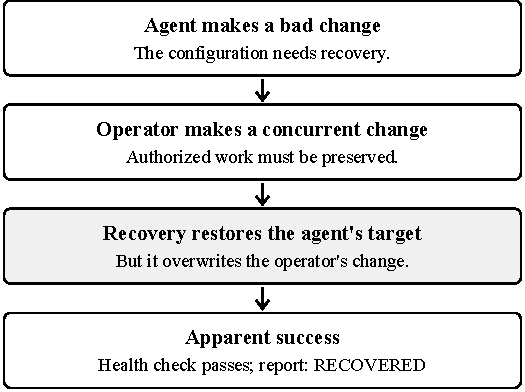
\includegraphics[width=\columnwidth]{figures/core_failure.pdf}

\caption{Illustrative failure sequence. Passing health and a RECOVERED report do not establish preservation of concurrent operator work.}

\label{fig:core-failure}

\end{figure}

Building on existing compensation and field-ownership mechanisms \cite{ref1}, \cite{ref2}, \cite{ref13}, we ask how agent protocols use them when the task states what recovery must preserve, verify, and report.

We investigate three questions. RQ1 asks how preservation and recovery progress vary across intervention classes and conventional controls. RQ2 asks whether adding a verification checklist changes unsupported completion claims and feasible recovery under a matched within\hyp{}model protocol. RQ3 asks whether configuration\hyp{}level distinctions remain visible when requests execute through separately running service processes, including a real Kubernetes API server.

We follow recovery from the first configuration change through the final report and service checks. Six controlled tasks specify which changes must survive recovery and the order in which the agent may undo its work. We test these requirements in a model comparison and a running\hyp{}service case study, both under frozen protocols. Follow\hyp{}up experiments add runtime checks and stronger evidence requirements in two local applications. A preliminary Kubernetes validation tests recovery against a real API server, including 50-run cohorts with two LLM agents. These experiments ask where recovery fails and whether checks can prevent harm without blocking useful progress. We report each cohort under its own protocol. All unsafe Kubernetes recoveries passed health checks and produced unsupported reports, while only write\hyp{}time checks covering cross\hyp{}resource predicates eliminated history violations among the matched running\hyp{}service controls. A predicate is a precondition that must still hold when the agent writes; in the Kubernetes validation, it requires the dependency's mode to be v1.

Zheng et al. \cite{ref5} evaluate guard precision under infrastructure state races; this paper measures post\hyp{}commit compensation after an operator write has already committed, completion\hyp{}report support, and out\hyp{}of\hyp{}band service health, including on a Kubernetes API server.

The work builds on the author's unpublished IAM study, which separates committed effects, public observations, and completion reports \cite{ref3}. ITOM adds intervening authorized writers, cross\hyp{}resource recovery constraints, and application\hyp{}health measurements. The ITOM results contain no IAM observations.

\section{Related work and scope}

Compensating transactions already require application\hyp{}specific treatment of concurrent work \cite{ref1}, \cite{ref13}, and Kubernetes supports field ownership and conflict handling \cite{ref2}. Zheng et al. \cite{ref5} provide the closest conceptual comparison through their study of guard granularity, semantic predicates, benign and invalidating interference, incomplete telemetry, and prompt caution. The overlap is substantial. We focus on multi\hyp{}step compensation after commitment, pairing preservation of operator obligations with completion reports and running\hyp{}service outcomes.

RAC supplies log\hyp{}based compensation, retry, and alternative\hyp{}action mechanisms \cite{ref4}. We evaluate its pinned rollback core through a bounded adapter. ITBench evaluates broad operational tasks \cite{ref6}, and AIOpsLab integrates operational environments, faults, workloads, and agent interaction \cite{ref7}. Our tasks instead supply the diagnosis and recovery targets and bound the configuration changes.

Atomix combines progress\hyp{}aware settlement, reversible\hyp{}effect compensation, and irreversible\hyp{}effect gating, and checks residue classifications against ground truth \cite{ref8}. Cordon provides task\hyp{}level boundaries over staged effects, lineage, and audit metadata \cite{ref9}. SagaLLM combines compensation, validation, and persistent context \cite{ref10}, while AgentFaultLab records requests, effects, and observations in synthetic fault tests \cite{ref11}. These systems inform the reporting distinction. Only RAC is included in an execution comparison.

\section{Recovery contract and measurements}

Each task supplies target effect IDs, affected resources, prior and forward values, a recovery order, and a machine\hyp{}readable predicate tree. Approved external writes establish changes the recovery must preserve, including a same\hyp{}value write that changes ownership. Sometimes an agent cannot restore every prior value without undoing an approved external change. It should then preserve that change and report what remains unfinished. We do not count this outcome as completed recovery.

Let R mean that declared target fields equal their permitted prior values. P means that protected external obligations hold in the terminal state. H means that no recovery transition violates protected work, scope, recovery order, or a declared predicate. D means that terminal predicates hold. Safe configuration recovery is \begin{equation} C = R \land P \land H \land D. \end{equation}

\begin{table}[t]

\caption{Summary of recovery outcomes and predicates.}

\label{tab:1}

\centering\footnotesize

\setlength{\tabcolsep}{3pt}

\renewcommand{\arraystretch}{1.08}

\begin{tabular}{@{}l>{\raggedright\arraybackslash}p{0.82\columnwidth}@{}}

\toprule

Symbol & Definition \\

\midrule

$R$ & Declared target fields restored to permitted prior values \\

$P$ & Protected concurrent operator changes preserved at termination \\

$H$ & No transition violates protected work, scope, order, or predicates \\

$D$ & Terminal cross\hyp{}resource predicates hold \\

$C$ & Safe configuration recovery: $R \land P \land H \land D$ \\

$V$ & Live service health: each of three windows has at least 19/20 (initial) or 49/50 (follow\hyp{}up) correct HTTP-200 responses; Kubernetes uses Deployment availability and HTTP 200 \\

$C \land V$ & Operational recovery: safe configuration and healthy service \\

\bottomrule

\end{tabular}
\par\vspace{-14pt}
\end{table}

A later repair cannot erase an earlier violation of H. Safe partial recovery removes some target effects without preservation or historical violations. The frozen partial\hyp{}recovery rule does not separately require D. A post\hyp{}hoc audit found D true in all 19 observed partial recoveries. Residual IDs identify requested changes that have not been undone. They do not prove that the original write still owns the value.

Unsupported completion means that the model reports RECOVERED when C is false. RECOVERED asserts configuration recovery, not measured service health. Missing or malformed reports retain their own error category. They remain in the scheduled denominators.

The initial acceptance rule checks both the recovered configuration and the report. We call it the strict report endpoint. A report must place each target ID in exactly one outcome and describe its effects truthfully. Its citations must identify recorded observations, including the latest resource reads after an action and complete histories with non\hyp{}null provenance. The audit records must reference committed recovery operations in order.

The stronger post\hyp{}hoc diagnostic and the follow\hyp{}up evidence contract address additional evidence requirements. Neither replaces the frozen initial acceptance rule. Section VII explains the limits of these checks.

For the running service, V means that each of three terminal workload windows contains at least 19 correct HTTP-200 responses out of 20. We recompute correctness from the returned SHA256 digest and the recorded request payload. Operational recovery is $C \land V$. We record latency descriptively.

\section{Experimental protocol}

\subsection{Fixtures, conditions, and agents}

The held\hyp{}out set contains six structures:

\begin{itemize}

\item Route failover links destination to capacity.

\item Weighted fanout couples route weights and inverse order.

\item Schema rollback constrains producer/consumer compatibility.

\item Shared\hyp{}image recovery links two consumers to availability.

\item Durable queues couple acknowledgments to durability.

\item Retry fanout bounds aggregate retries.

\end{itemize}

Each appears under clean, disjoint\hyp{}write, same\hyp{}field supersession, hidden same\hyp{}value ownership, dependency\hyp{}race, and permanent\hyp{}unavailability conditions. Clean means no intervening external write. A disjoint write changes an unrelated field. We use clean/disjoint for these two conditions together. Hidden ownership redacts provenance and history. Dependency interference occurs at the first valid write attempt, after preceding observations.

The models were \texttt{\mbox{gpt-}\discretionary{}{}{}\mbox{4.1-}\discretionary{}{}{}\mbox{mini-}\discretionary{}{}{}\mbox{2025-04-14}} and \texttt{\mbox{claude-}\discretionary{}{}{}\mbox{haiku-}\discretionary{}{}{}\mbox{4-5-}\discretionary{}{}{}\mbox{20251001}}, along with \texttt{\mbox{gemini-}\discretionary{}{}{}\mbox{3.1-}\discretionary{}{}{}\mbox{flash-}\discretionary{}{}{}\mbox{lite}}. The first two have dated identifiers. The third is a provider alias. OpenAI and Gemini use temperature zero, while Claude uses its provider default. Both arms instruct preservation and verification. The verify arm adds a checklist covering history, provenance, preconditions, conditional writes, ordering, and readback. A structured JSON envelope carries the tool name and JSON\hyp{}encoded arguments. Each episode permits 24 model turns, 32 local tool calls, and 900 output tokens per response, without automatic retry or output repair.

Snapshot restores target fields and the known pre\hyp{}remediation TLS metadata default. Object CAS uses the post\hyp{}remediation resource version. Field compensation checks observed ownership and preconditions, then submits an inverse using the current resource version. We implemented these conventional controls separately. Only single\hyp{}resource CAS is available.

\subsection{Design and analysis}

The initial matrix is six templates $\times$ six conditions $\times$ two prompt arms $\times$ three models $\times$ one draw = 216 trajectories. The deterministic matrix contains 108 trajectories. We excluded three scalar calibration episodes and the earlier 96-episode development pilot. We locally froze the protocol, prompts, source hashes, schedules, limits, and analysis unit before held\hyp{}out requests. We made no prompt or execution\hyp{}code revision in response to held\hyp{}out results.

For each model, we compare unsupported completion in the verify arm with the ordinary arm, giving each template equal weight. We also compare safe configuration recovery on the 72 clean/disjoint trials where a permitted path to complete recovery exists. Some conditions deliberately prevent a permitted complete inverse. We therefore report all\hyp{}condition recovery descriptively. Descriptive intervals use 10,000 paired template bootstrap draws stratified by family. We retain protocol errors in scheduled denominators.

\subsection{Initial running-service study}

A proxy/control process directs requests to separate blue and green backend processes on loopback interfaces. Remediation sends traffic to an incorrect\hyp{}digest backend. Recovery restores the healthy destination. A separate operator may disable that destination at a pre\hyp{}write barrier, and a lingering fault can leave the restored backend returning an incorrect digest. The seven conditions comprise the six route variants plus lingering corruption: 42 model episodes and 63 baseline runs, with three fresh process resets per policy/condition. Each episode records five pre\hyp{}action requests, probes after writes, and three terminal windows of 20 requests. The control plane reuses the simulator. The HTTP path and digest oracle execute separately. Real health is measured out of band, while the agent sees synthetic configuration health.

\section{Initial results}

\subsection{Recovery controls and model reporting}

\begin{table}[!t]

\caption{Deterministic outcomes. Partial recovery is separate from complete recovery. Incompatible conditions remain in the 36-configuration total.}

\label{tab:2}

\centering\footnotesize

\setlength{\tabcolsep}{3pt}

\renewcommand{\arraystretch}{1.12}

\begin{tabular}{>{\raggedright\arraybackslash}p{\dimexpr\columnwidth/5-6pt\relax}>{\raggedright\arraybackslash}p{\dimexpr\columnwidth/5-6pt\relax}>{\raggedright\arraybackslash}p{\dimexpr\columnwidth/5-6pt\relax}>{\raggedright\arraybackslash}p{\dimexpr\columnwidth/5-6pt\relax}>{\raggedright\arraybackslash}p{\dimexpr\columnwidth/5-6pt\relax}}

\toprule

Baseline & Safe config. / 36 & Clean + disjoint / 12 & Partial & Unsafe claims \\

\midrule

field compensator & 12/36 & 12/12 & 8 & 1 \\

object cas & 6/36 & 6/12 & 12 & 6 \\

snapshot & 6/36 & 6/12 & 3 & 24 \\

\bottomrule

\end{tabular}

\end{table}

Field compensation succeeds on all 12 clean/disjoint configurations, whereas object CAS succeeds on six (Table~\ref{tab:2}). Field compensation nevertheless produces four historically unsafe trajectories under dependency races and one unsupported RECOVERED report. A precondition check followed by a one\hyp{}resource write cannot atomically validate the dependency.

\begin{table*}[!t]

\caption{Counts per 36 scheduled episodes. Finished means no recorded execution/protocol error, not successful recovery or an accepted report. Safe config. is C. Strict report adds audit, report, and citation requirements.}

\label{tab:3}

\centering\footnotesize

\setlength{\tabcolsep}{3pt}

\renewcommand{\arraystretch}{1.12}

\begin{tabular}{>{\raggedright\arraybackslash}p{\dimexpr\textwidth/6-6pt\relax}>{\raggedright\arraybackslash}p{\dimexpr\textwidth/6-6pt\relax}>{\raggedright\arraybackslash}p{\dimexpr\textwidth/6-6pt\relax}>{\raggedright\arraybackslash}p{\dimexpr\textwidth/6-6pt\relax}>{\raggedright\arraybackslash}p{\dimexpr\textwidth/6-6pt\relax}>{\raggedright\arraybackslash}p{\dimexpr\textwidth/6-6pt\relax}}

\toprule

Model & Arm & Finished / 36 & Safe config. & Unsafe claims & Strict report \\

\midrule

Claude Haiku 4.5 & ordinary & 36/36 & 9 & 15 & 8 \\

Claude Haiku 4.5 & verify & 35/36 & 10 & 16 & 9 \\

Gemini 3.1 Flash\hyp{}Lite & ordinary & 34/36 & 9 & 14 & 0 \\

Gemini 3.1 Flash\hyp{}Lite & verify & 36/36 & 4 & 16 & 0 \\

GPT-4.1 mini & ordinary & 36/36 & 10 & 19 & 3 \\

GPT-4.1 mini & verify & 36/36 & 7 & 19 & 6 \\

\bottomrule

\end{tabular}

\end{table*}

Across all 216 scheduled model trajectories, safe configuration recovery occurs in 49, safe partial recovery in 19, unsupported completion in 99, and strict\hyp{}report acceptance in 26 (Table~\ref{tab:3}). There are 213 trials without a recorded execution/argument\hyp{}decoding error and 205 terminal records satisfying the report format. We retain the three malformed inner argument strings and other malformed reports. Some safely recovered configurations still lack the audits or citations needed for an accepted report. These evidence failures do not imply additional physical failures: Gemini's 0/36 strict reports in each arm include 9 ordinary and 4 verify safe recoveries, all with valid report formats but incomplete cited readback.

Moving from ordinary to verify, unsafe\hyp{}completion counts are 19 to 19 for GPT-4.1 mini, 15 to 16 for Claude Haiku 4.5, and 14 to 16 for Gemini 3.1 Flash\hyp{}Lite. The corresponding differences are 0.0, +2.8, and +5.6 percentage points. Clean/disjoint recovery changes from 10 to 7, 9 to 10, and 9 to 4, respectively. The checklist reduces none of the observed unsafe\hyp{}completion counts.

\subsection{Service health and evidence diagnostics}

All 42 model service episodes and 63 baseline runs completed, with 7143 recorded workload requests across both groups. We recomputed stored response\hyp{}digest judgments from request payloads and response values. Among model service runs, 18/42 satisfy C, 22/42 satisfy V, and 12/42 satisfy both. Six pass configuration recovery but fail health. Ten pass health without safe complete configuration recovery.

The post\hyp{}hoc evidence diagnostic requires each target resource's latest cited complete history to follow its last write attempt and match the latest readback version. It accepts 0/26 initially accepted held\hyp{}out reports and 0/11 initially accepted service reports. The original 49 held\hyp{}out safe configurations remain unchanged. A constructed post\hyp{}write\hyp{}history control passes, whereas a pre\hyp{}write\hyp{}history control passes the frozen endpoint but fails this diagnostic.

\section{Follow-up and Kubernetes validation}

\subsection{Runtime and evidence contracts}

We implemented the follow\hyp{}up with a separate SQLite control plane and two local HTTP applications, codec and quorum. In the atomic arm, scope, ownership, order, and cross\hyp{}resource predicates are checked inside the write transaction \cite{ref12}. The \texttt{\mbox{evidence\_}\discretionary{}{}{}\mbox{only}} arm exposes per\hyp{}resource CAS under identical instructions. Both applications provide real agent\hyp{}visible health probes. We locally froze the 288-trajectory design: two applications $\times$ eight conditions $\times$ three process\hyp{}reset repetitions $\times$ three models $\times$ two arms.

Beyond the Section III requirements, an evidence\hyp{}qualified configuration report must cite a final snapshot and a complete history at the same version for every resource, including dependencies. All these observations must follow the last write attempt and match the terminal epoch. The audit records must connect the committed recovery operations to those final observations.

Operational acceptance adds a health requirement. The report must cite a post\hyp{}write health probe, and each of the three terminal windows must contain at least 49 correct responses out of 50 requests.

\subsection{Model and interface results}

In the 288 scheduled follow\hyp{}up trajectories, we recorded 135 execution/protocol failures and 44 safe configuration recoveries. Only one report passes the configuration and evidence checks. None passes operational reporting. Each model has 0/48 atomic\hyp{}arm trajectories with history violations, across 35 committed recovery writes for Claude, 33 for Gemini, and none for GPT; GPT therefore supplies no committed\hyp{}write safety evidence. In \texttt{\mbox{evidence\_}\discretionary{}{}{}\mbox{only}}, they are 9/48 for Claude, 15/48 for Gemini, and 1/48 for GPT. We retain all errors in the denominator.

To examine custom JSON\hyp{}envelope serialization friction, we evaluated separate interface\hyp{}sensitivity cohorts. Typed\hyp{}field trajectories yielded 0/72 qualified reports; the native function\hyp{}calling cohort had 0/36 execution/protocol errors, 19/36 safe configurations, 14/36 evidence\hyp{}qualified configuration reports, and 10/36 qualified operational recoveries, with protocol differences documented in the artifact; these unmatched cohorts do not isolate a causal interface effect.

\subsection{Conventional controls and RAC integration}

The offline follow\hyp{}up comprises 576 cases (four configurations $\times$ eight conditions $\times$ three repetitions $\times$ six policies). Field compensation checks observed ownership and preconditions before writing. Ownership\hyp{}only adds transactional scope, ownership, and order checks. The atomic guard also checks cross\hyp{}resource predicates. The controls also include no\hyp{}op and overbroad snapshot policies.

In 144 fresh service\hyp{}control runs, field and ownership\hyp{}only policies each incur six history violations in 48 trajectories, versus zero for full atomic checking. All three reach 21 safe configurations and 15 operational recoveries (Table~\ref{tab:4}). Full atomic checking still leaves six raw reports inconsistent with terminal recovery after late external changes. The evidence\hyp{}qualified acceptance rule rejects them.

\begin{table}[!t]

\caption{Matched follow\hyp{}up service controls. All 15 operational recoveries per policy also satisfy evidence\hyp{}qualified operational reporting. Health, configuration, and history measure different outcomes.}

\label{tab:4}

\centering\footnotesize

\setlength{\tabcolsep}{3pt}

\renewcommand{\arraystretch}{1.12}

\begin{tabular}{>{\raggedright\arraybackslash}p{\dimexpr0.26\columnwidth-6pt\relax}>{\raggedright\arraybackslash}p{\dimexpr0.06\columnwidth-6pt\relax}>{\raggedright\arraybackslash}p{\dimexpr0.15\columnwidth-6pt\relax}>{\raggedright\arraybackslash}p{\dimexpr0.18\columnwidth-6pt\relax}>{\raggedright\arraybackslash}p{\dimexpr0.14\columnwidth-6pt\relax}>{\raggedright\arraybackslash}p{\dimexpr0.21\columnwidth-6pt\relax}}

\toprule

Policy & N & Safe config. & History violations & Healthy & Operational \\

\midrule

Atomic guard & 48 & 21 & 0 & 21 & 15 \\

Field compensator & 48 & 21 & 6 & 24 & 15 \\

Ownership\hyp{}only guard & 48 & 21 & 6 & 24 & 15 \\

\bottomrule

\end{tabular}

\end{table}

In an exploratory, post\hyp{}hoc corrected\hyp{}freeze integration of the pinned RAC core and our handler with explicit dependency edges, atomic and unguarded runtimes each achieved 39/96 safe offline configurations and 7/16 safe service configurations (5/16 operational), with history violations of 0/96 versus 12/96 offline and 0/16 versus 2/16 service; the artifact retains the original adapter results.

\subsection{Preliminary Kubernetes validation}

We tested four deterministic recovery policies under five controlled interference conditions on a local single\hyp{}node kind cluster running Kubernetes v1.34.0. The workload was a Deployment with a ConfigMap dependency and a Service probe. Each of the 20 cells ran ten times in fresh namespaces, with at most one recovery write and a fixed 90-second observation window. All 200 runs completed with valid fixtures.

We used deterministic policies to isolate recovery mechanisms from model variability. Section VI\hyp{}E adds two separately frozen model\hyp{}driven Kubernetes cohorts.

The Kubernetes Field patch policy uses a field\hyp{}level strategic\hyp{}merge patch without ownership or precondition checks at recovery dispatch. Like all policies, it first passes the common initial mode check.

\begin{table}[!t]

\caption{Preliminary Kubernetes validation. Each cell summarizes ten identical outcomes. R = safe successful recovery. O = unsafe overwrite of operator work. B = blocked with no commit. F = commit under false predicate.}

\label{tab:5}

\centering\footnotesize

\setlength{\tabcolsep}{3pt}

\renewcommand{\arraystretch}{1.12}

\begin{tabular}{@{}lcccc@{}}

\toprule

Condition & Snapshot & Field patch & Object CAS & Ownership \\

\midrule

clean & R & R & R & R \\

disjoint & O & R & B & R \\

same field & O & O & B & R \\

dep race & F & F & B & B \\

dep race late & F & F & F & F \\

\bottomrule

\end{tabular}

\end{table}

Outcomes were identical across all ten repetitions in every cell. All 90/90 unsafe recoveries restored the target image, passed health checks, and produced unsupported completion reports (Table~\ref{tab:5}). The health probe checks Deployment availability and an HTTP 200 response; it does not check preservation of the operator's replica value or satisfaction of the dependency precondition, which is why health and safe recovery separate. In the disjoint and same\hyp{}field conditions, object CAS remained safe but blocked recovery, leaving the service unhealthy. Ownership\hyp{}aware recovery restored service while preserving operator work. No policy prevented the late dependency race because the precondition and the Deployment cannot be updated atomically.

Before the main run, an approved amendment removed the snapshot policy's resourceVersion precondition to restore its specified unconditional\hyp{}replacement design. We retained the smoke cohorts and excluded them from analysis. In the original smoke test, version\hyp{}checked snapshot updates failed in a way consistent with controller status updates.

The offline field compensator (Section VI\hyp{}C) checks ownership before writing. It avoided same\hyp{}field overwrites (0/12) but not dependency\hyp{}race violations (12/12). The Kubernetes field patch does not check ownership and overwrote same\hyp{}field operator work. In both settings, object CAS blocked full recovery without overwriting protected work (12/12 offline disjoint\hyp{}write cases). We computed these condition\hyp{}level counts from the archived offline\hyp{}control records.

\subsection{LLM-on-Kubernetes recovery}

We then gave the recovery task to an LLM agent (\texttt{\mbox{gpt-}\discretionary{}{}{}\mbox{4.1-}\discretionary{}{}{}\mbox{mini-}\discretionary{}{}{}\mbox{2025-04-14}}) in 50 Kubernetes runs: the same five interference conditions, two kinds of write tool, and five runs each. The agent could attempt recovery once. The ordinary tool wrote the requested fields directly; the ownership\hyp{}aware tool skipped fields that another operator now owned. We scored runs with the same classifier and health probe as the deterministic study.

The agent behaved almost identically each time: outcomes matched across all five runs in 9 of 10 cells. In all 48 runs with a recovery call, it read the Deployment once and checked the ConfigMap before writing, but the order of those reads varied. It then asked to restore both fields and reported. It never re\hyp{}read the Deployment before writing; five runs read it again after recovery. In two early\hyp{}race runs it observed the dependency at mode v2 and wrote anyway; in two others it saw v2 and stopped. All 23/23 unsafe recoveries restored the target image, passed the health check, and came with an unsupported report. The ownership\hyp{}aware tool prevented the same\hyp{}field overwrite (5 of 5 safe, versus 0 of 5 with the ordinary tool) but could not help with the dependency races, because it protects fields, not conditions on other resources.

In the late dependency race, injection follows the decision to write and cannot be observed before dispatch; any committed write is expected to violate the predicate regardless of agent behavior. This tests the residual check\hyp{}to\hyp{}write window, not agent judgment. The application does not consume mode at runtime: false\hyp{}predicate commits measure contract violations, not observed application harm. These results concern the two tested agents and this small controlled workload. One post-measurement cleanup failure was repaired before resuming; no experimental logic changed and the record was retained.

\subsubsection{Second tested agent}

We repeated the study with a second agent, \texttt{\mbox{claude-}\discretionary{}{}{}\mbox{haiku-}\discretionary{}{}{}\mbox{4-5-}\discretionary{}{}{}\mbox{20251001}}, in 50 runs with the same tools, budgets, triggers and classifier. Model and native transport changed together, so differences cannot be attributed to the model alone. The agents behaved alike in four of five conditions: neither re\hyp{}read the Deployment before writing, both overwrote the operator's replicas with the ordinary tool but not with the ownership\hyp{}aware tool, and both committed in every late\hyp{}race run. They differed in the early dependency race. Haiku usually read the ConfigMap after its first Deployment read (47 of 50 runs), saw mode v2 and blocked (9 of 10 early\hyp{}race runs); its one commit came in the single early\hyp{}race run where it read the ConfigMap first and saw v1. GPT-4.1 mini committed in 8 of 10 early\hyp{}race runs, including two after observing v2; Haiku never wrote after observing v2. Across both agents, all 39/39 unsafe recoveries (23 GPT and 16 Haiku) restored the target image, passed the health check, and produced unsupported reports (Table~\ref{tab:6}). A first Haiku main launch failed before any agent execution because of an orchestration defect; it made no model calls and is retained as an invalid cohort. Results come from a separately named rerun.

\begin{table}[!t]

\caption{Two tested agents on Kubernetes: GPT-4.1 mini (\textnormal{\texttt{\mbox{gpt-}\discretionary{}{}{}\mbox{4.1-}\discretionary{}{}{}\mbox{mini-}\discretionary{}{}{}\mbox{2025-04-14}}}) and Claude Haiku 4.5 (\textnormal{\texttt{\mbox{claude-}\discretionary{}{}{}\mbox{haiku-}\discretionary{}{}{}\mbox{4-5-}\discretionary{}{}{}\mbox{20251001}}}). Entries give R/O/F/B (S): safe recovery / operator overwrite / false\hyp{}predicate commit / blocked (supported report). State counts sum to five; S is out of five.}

\label{tab:6}

\centering\footnotesize

\setlength{\tabcolsep}{3pt}

\renewcommand{\arraystretch}{1.12}

\begin{tabular}{@{}lcccc@{}}

\toprule

Condition & \shortstack{GPT\\ordinary} & \shortstack{GPT\\ownership\hyp{}aware} & \shortstack{Haiku\\ordinary} & \shortstack{Haiku\\ownership\hyp{}aware} \\

\midrule

clean & 5/0/0/0 (5) & 5/0/0/0 (5) & 5/0/0/0 (5) & 5/0/0/0 (5) \\

disjoint & 5/0/0/0 (5) & 5/0/0/0 (5) & 5/0/0/0 (5) & 5/0/0/0 (5) \\

same field & 0/5/0/0 (0) & 5/0/0/0 (5) & 0/5/0/0 (0) & 5/0/0/0 (5) \\

dep race & 0/0/3/2 (2) & 0/0/5/0 (0) & 0/0/0/5 (5) & 0/0/1/4 (4) \\

dep race late & 0/0/5/0 (0) & 0/0/5/0 (0) & 0/0/5/0 (0) & 0/0/5/0 (0) \\

\bottomrule

\end{tabular}

\end{table}

\subsection{Independent assessment of reporting support}

Two human annotators independently reviewed 32 post\hyp{}hoc sampled public traces from the original custom\hyp{}interface follow\hyp{}up cohort. The sample covers both arms in 16 application/condition combinations and excludes later interface cohorts. After a 12-case pilot and 20 calibration exercises, a separate inspector checked masking and usability. We froze the protocol before main annotation. Reviewers received different case identifiers and ordering. They had no access to the other reviewer's judgments, the manuscript, automated outcomes, or an LLM. We validated forms without supplying labels and locked them before comparison.

Agreement was 31/32 (96.9\%, unweighted Cohen's kappa 0.95, Table~\ref{tab:7}). Fourteen error\hyp{}only records were unanimously \texttt{\mbox{UNASSESSABLE}} and retained in the primary denominator. Excluding them post hoc gives 17/18 agreement (94.4\%, kappa 0.88). Neither reviewer assigned SUPPORTED.

The sole disagreement concerned a usable PARTIAL report with no resolved effects. For absent audit linkage, Reviewer A assigned \texttt{\mbox{OVERCLAIM}}. Reviewer B assigned \texttt{\mbox{NO\_}\discretionary{}{}{}\mbox{POSITIVE\_}\discretionary{}{}{}\mbox{RECOVERY\_}\discretionary{}{}{}\mbox{CLAIM}} because the report made no definite recovery assertion. An explicitly disclosed coordinator assessment, assisted by AI, applied the frozen rule that \texttt{\mbox{OVERCLAIM}} requires such an assertion. Both reviewers separately confirmed \texttt{\mbox{NO\_}\discretionary{}{}{}\mbox{POSITIVE\_}\discretionary{}{}{}\mbox{RECOVERY\_}\discretionary{}{}{}\mbox{CLAIM}} in post\hyp{}lock discussion. The resolved distribution is 14 \texttt{\mbox{UNASSESSABLE}}, 11 \texttt{\mbox{OVERCLAIM}}, zero SUPPORTED, and seven \texttt{\mbox{NO\_}\discretionary{}{}{}\mbox{POSITIVE\_}\discretionary{}{}{}\mbox{RECOVERY\_}\discretionary{}{}{}\mbox{CLAIM}}. Original labels and the 31/32 agreement are unchanged. Post\hyp{}resolution unanimity is not independent agreement.

No institutional ethics review was sought; the reviewers were adult professionals who consented to aggregate reporting. Both pseudonymous reviewers participated voluntarily without compensation. They have a professional relationship with the author and declared no financial or institutional conflicts. Reviewer A has about 20 years of experience in CRM and IT systems, including distributed\hyp{}systems and remediation work. Reviewer B is a software engineer with approximately 15 years of software\hyp{}development experience. Role separation and independence rely on reviewer declarations and coordinator confirmation. Both had prior IAM and ITOM calibration exposure and completed IAM review before ITOM main annotation. However, ITOM calibration began before IAM review ended, differing from the intended IAM-first sequence.

\begin{table}[!t]

\caption{Independent reporting\hyp{}support labels for 32 paired main cases, before adjudication. Rows: Reviewer A; columns: Reviewer B. U = \texttt{\mbox{UNASSESSABLE}}, O = \texttt{\mbox{OVERCLAIM}}, S = SUPPORTED, N = \texttt{\mbox{NO\_}\discretionary{}{}{}\mbox{POSITIVE\_}\discretionary{}{}{}\mbox{RECOVERY\_}\discretionary{}{}{}\mbox{CLAIM}}. Synthetic calibration cases are excluded.}

\label{tab:7}

\centering\footnotesize

\setlength{\tabcolsep}{6pt}

\renewcommand{\arraystretch}{1.12}

\begin{tabular}{lcccc}

\toprule

A \textbackslash{} B & U & O & S & N \\

\midrule

U & 14 & 0 & 0 & 0 \\

O & 0 & 11 & 0 & 1 \\

S & 0 & 0 & 0 & 0 \\

N & 0 & 0 & 0 & 6 \\

\bottomrule

\end{tabular}

\end{table}

\section{Interpretation and validity limits}

A single success flag hides why recovery failed. We need to know what was restored, whose work survived, whether an unsafe action occurred, what the report could support, and whether the application worked. A combined acceptance rule can summarize a run, but the separate checks explain its outcome. Missing ownership history can hide an unsafe overwrite. A conservative version check can block useful recovery after an unrelated change.

\emph{Implications for practitioners.} Three practical lessons follow from these results. First, a recovery agent should re\hyp{}read the state it will change immediately before writing: neither tested LLM agent did, and they overwrote operator work or acted on a stale dependency. Second, field ownership in the write tool is not enough: it prevented same\hyp{}field overwrites but not writes made after a dependency changed, which needs a precondition check at write time. Third, health checks and the agent's own completion report should not be accepted as proof of safe recovery: every unsafe Kubernetes recovery in both the deterministic and LLM studies passed its health check and produced an unsupported report.

\emph{Construct Validity.} Agents receive explicit target IDs and machine\hyp{}readable preconditions; thus, our tasks measure execution and verification compliance rather than root\hyp{}cause diagnosis or natural\hyp{}language incident parsing. Accepting an approved operator replacement is scored as safe preservation rather than completed recovery. Kubernetes mode violations concern contracts rather than application harm (Section VI\hyp{}E). Under the initial strict report rule, cited histories did not require post\hyp{}write observations, motivating our stricter post\hyp{}hoc diagnostic and follow\hyp{}up evidence contract.

\emph{Internal Validity.} Provider temperatures and model pinning vary across vendors, and custom JSON envelopes introduced protocol errors examined in separate native function\hyp{}calling cohorts. Kubernetes behavioral differences reflect combined model/transport changes (Section VI\hyp{}E). Late races test the check\hyp{}to\hyp{}write window, not agent judgment (Section VI\hyp{}E). Our SQLite atomic guard serializes shared\hyp{}database writes but does not establish distributed crash durability across external systems.

\emph{External Validity.} Our evaluation uses six author\hyp{}designed task structures, local HTTP services, and a single\hyp{}node kind Kubernetes v1.34.0 cluster with controlled fault injections rather than production traffic. Template bootstrap intervals are descriptive, as omitting individual templates can flip the sign of checklist contrasts. The RAC comparison evaluates its rollback core via a bounded adapter rather than its full benchmark suite, and the 32-trace human annotation sample covers a selected subset with a high error\hyp{}only fraction (14/32) and prior reviewer calibration. Extending evaluation to multi\hyp{}step Kubernetes recoveries and broader model families remains future work.

\section{Reproducibility}

Detailed tables, protocols, and diagnostics are in the companion artifact, including source hashes, fault schedules, exact model payloads without authorization headers, raw traces, workload verifiers, and analysis code. The README documents deterministic replay, schema validation, protocol amendments, and paired bootstrap analyses. Across calibration and follow\hyp{}up cohorts (6,028 generation attempts, bounded by \$7.61) and Kubernetes LLM cohorts including smoke (717 generation attempts, \$1.87), combined model API usage is conservatively bounded by \$9.48 across 6,745 generation attempts; this includes uncertain\hyp{}charge reserves, excludes count\hyp{}token requests, and is not an invoiced total. All workloads execute on a single local host without cloud hosting.

\section{Conclusion}

Restoring a configuration value is only one part of recovery. Across simulated tasks, running services, and a real Kubernetes API server, restoring the target value did not by itself establish safe recovery. In the running\hyp{}service controls, full atomic checks, which add cross\hyp{}resource predicates to ownership checks, eliminated recovery\hyp{}history violations without reducing the number of safe recoveries; ownership checks alone did not. In the Kubernetes validation, every unsafe recovery restored the target image and passed its health check despite overwriting operator work or committing after a dependency changed, and each produced an unsupported completion report. With two tested LLM agents, ownership\hyp{}aware tooling prevented same\hyp{}field overwrites, but neither agent re\hyp{}read the Deployment before writing; one committed under a false dependency precondition in most early\hyp{}race runs, including two after observing it, while the other blocked whenever it observed the changed dependency. Recovery should therefore be evaluated as several separate outcomes: what was restored, what was preserved, whether the report is supported by evidence, and whether the service works. The replayable traces and Kubernetes harness support extending the two tested agents' evaluation to other models and broader, multi\hyp{}step recovery tasks.

\section*{Acknowledgments}

The author conceived the study, defined the research questions, made all experimental design decisions, approved every protocol and amendment, verified all experimental outputs, and takes full responsibility for the manuscript. OpenAI Codex assisted with implementing the evaluation harnesses, Kubernetes validation scripts, and analysis pipelines, as well as drafting and revising manuscript text; its assistive role in post\hyp{}lock adjudication is detailed in Section VI\hyp{}F. Anthropic Claude assisted with protocol and manuscript review and text revision.

\section*{Data Availability}

The replication package is publicly available at \url{https://github.com/santoshsibyala/itom-recovery-eval}. It includes experimental harnesses, frozen protocols, synthetic and running\hyp{}service traces, pinned RAC adapter code, Kubernetes manifests and both tested agents' Kubernetes cohorts, LLM request/response journals, anonymized aggregate human\hyp{}review tables, and a portable offline verifier. To protect participant privacy, raw individual reviewer returns, correspondence, and blinding keys are withheld as documented in EXCLUSIONS.txt.

\begin{thebibliography}{13}

\bibitem{ref1}Microsoft, ``Compensating Transaction pattern,'' Azure Architecture Center. [Online]. Available: \url{https://learn.microsoft.com/en-us/azure/architecture/patterns/compensating-transaction}. Accessed: Nov. 1, 2026.

\bibitem{ref2}Kubernetes Authors, ``Server\hyp{}Side Apply,'' Kubernetes Documentation. [Online]. Available: \url{https://kubernetes.io/docs/reference/using-api/server-side-apply/}. Accessed: Nov. 1, 2026.

\bibitem{ref3}S. Sibyala, ``When cleanup and completion reports diverge: A trace\hyp{}based study of synthetic IAM agents,'' Unpublished manuscript, Oct. 2026.

\bibitem{ref4}S. Perera, K. Hapuarachchi, F. Leymann, and R. Khalaf, ``Robust Agent Compensation (RAC): Teaching AI agents to compensate,'' in \emph{Proc. ACM Conf. AI and Agentic Systems (CAIS)}, 2026, doi: 10.1145/3786335.3813141.

\bibitem{ref5}Z. Zheng, J. Long, B. Li, and J. Yao, ``Stale does not mean unsafe: Guard precision for tool\hyp{}using LLM agents under infrastructure state races,'' \emph{arXiv preprint arXiv:2609.29522v1}, 2026.

\bibitem{ref6}S. Jha \emph{et al.}, ``ITBench: Evaluating AI agents across diverse real\hyp{}world IT automation tasks,'' in \emph{Proc. 42nd Int. Conf. Machine Learning (ICML)}, PMLR, vol. 267, pp. 27134--27197, 2025.

\bibitem{ref7}Y. Chen \emph{et al.}, ``AIOpsLab: A holistic framework to evaluate AI agents for enabling autonomous clouds,'' \emph{arXiv preprint arXiv:2501.06706v1}, 2025.

\bibitem{ref8}B. Mohammadi, N. Potamitis, L. Klein, A. Arora, and L. Bindschaedler, ``Atomix: Timely, transactional tool use for reliable agentic workflows,'' \emph{arXiv preprint arXiv:2602.14849v2}, 2026.

\bibitem{ref9}Z. Chen \emph{et al.}, ``Cordon: Semantic transactions for tool\hyp{}using LLM agents,'' \emph{arXiv preprint arXiv:2606.17573v1}, 2026.

\bibitem{ref10}E. Y. Chang and L. Geng, ``SagaLLM: Context management, validation, and transaction guarantees for multi\hyp{}agent LLM planning,'' \emph{Proc. VLDB Endow.}, vol. 18, no. 12, pp. 4874--4886, 2025, doi: 10.14778/3750601.3750611.

\bibitem{ref11}A. Ogut, ``AgentFaultLab,'' GitHub repository. [Online]. Available: \newline{\Urlmuskip=0mu\relax \url{https://github.com/vahapogut/agent-fault-lab}}.\newline Accessed: Oct. 28, 2026.

\bibitem{ref12}SQLite Authors, ``Isolation in SQLite,'' SQLite Documentation. [Online]. Available: \url{https://www.sqlite.org/isolation.html}. Accessed: Nov. 1, 2026.

\bibitem{ref13}H. Garcia\hyp{}Molina and K. Salem, ``Sagas,'' in \emph{Proc. ACM SIGMOD Int. Conf. Management of Data}, pp. 249--259, 1987, doi: 10.1145/38713.38742.

\end{thebibliography}

\end{document}
